\documentclass{beamer}

\usepackage{aula}

\title{Geoprocessamento}
\date{\today}

\begin{document}
    
\input{capa}



\begin{frame}[fragile]{ST\_Intersects — Interseção}
    
    Retorna verdadeiro se duas geometrias possuem qualquer interseção.
    
    \begin{minted}{sql}
SELECT *
FROM cidades c, estados e
WHERE ST_Intersects(c.geom, e.geom);
    \end{minted}
    
    \begin{center}
        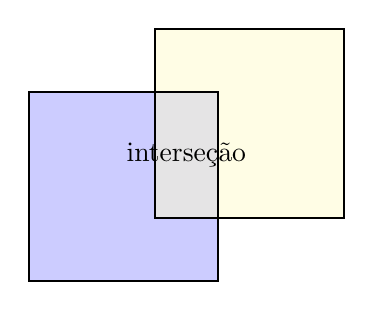
\begin{tikzpicture}[scale=0.8]
            
            \draw[fill=blue!20] (0,0) rectangle (3,3);
            \draw[opacity=.5,fill=yellow!20] (2,1) rectangle (5,4);
            
            \draw[thick] (0,0) rectangle (3,3);
            \draw[thick] (2,1) rectangle (5,4);
            
            \node at (2.5,2) {interseção};
            
        \end{tikzpicture}
    \end{center}
    
\end{frame}

\begin{frame}[fragile]{ST\_Contains — Contém}
    
    Retorna verdadeiro se uma geometria está completamente dentro de outra.
    
    \begin{minted}{sql}
SELECT *
FROM estados e, cidades c
WHERE ST_Contains(e.geom, c.geom);
    \end{minted}
    
    \begin{center}
        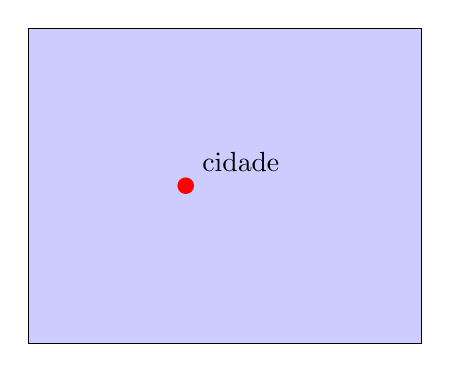
\begin{tikzpicture}
            
            \draw[fill=blue!20] (0,0) rectangle (5,4);
            \fill[red] (2,2) circle (3pt);
            
            \node at (2.7,2.3) {cidade};
            
        \end{tikzpicture}
    \end{center}
    
\end{frame}

\begin{frame}[fragile]{ST\_Within — Está dentro}
    
    Equivalente lógico de \texttt{ST\_Contains} invertido.
    
    \begin{minted}{sql}
SELECT *
FROM cidades c, estados e
WHERE ST_Within(c.geom, e.geom);
    \end{minted}
    
    \begin{center}
        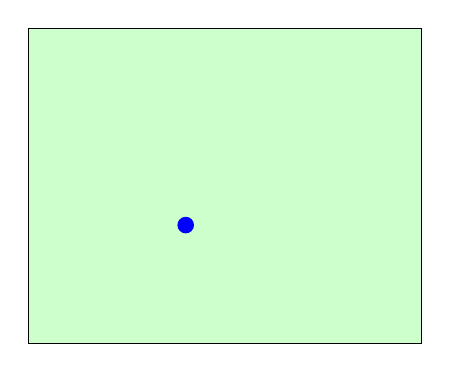
\begin{tikzpicture}
            
            \draw[fill=green!20] (0,0) rectangle (5,4);
            \fill[blue] (2,1.5) circle (3pt);
            
        \end{tikzpicture}
    \end{center}
    
\end{frame}

\begin{frame}[fragile]{ST\_Touches — Toque}
    
    Geometrias compartilham borda mas não área interna.
    
    \begin{minted}{sql}
SELECT *
FROM municipios a, municipios b
WHERE ST_Touches(a.geom, b.geom);
    \end{minted}
    
    \begin{center}
        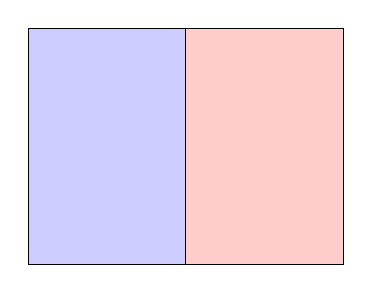
\begin{tikzpicture}
            
            \draw[fill=blue!20] (0,0) rectangle (2,3);
            \draw[fill=red!20] (2,0) rectangle (4,3);
            
        \end{tikzpicture}
    \end{center}
    
\end{frame}

\begin{frame}[fragile]{ST\_Overlaps — Sobreposição}
    
    As geometrias se sobrepõem parcialmente.
    
    \begin{minted}{sql}
SELECT *
FROM uso_solo a, uso_solo b
WHERE ST_Overlaps(a.geom, b.geom);
    \end{minted}
    
    \begin{center}
        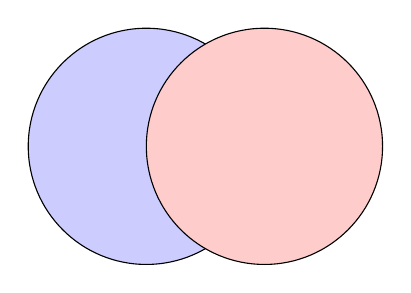
\begin{tikzpicture}
            
            \draw[fill=blue!20] (0,0) circle (1.5);
            \draw[fill=red!20] (1.5,0) circle (1.5);
            
        \end{tikzpicture}
    \end{center}
    
\end{frame}

\begin{frame}[fragile]{ST\_Buffer — Zona de influência}
    
    Cria uma área ao redor de uma geometria.
    
    \begin{minted}{sql}
SELECT ST_Buffer(geom, 1000)
FROM rios;
    \end{minted}
    
    \begin{center}
        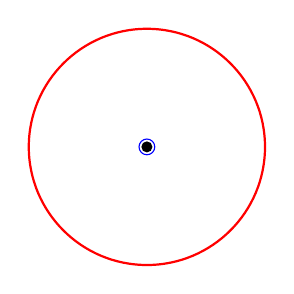
\begin{tikzpicture}
            
            \fill (0,0) circle (2pt);
            \draw[blue] (0,0) circle (0.1);
            \draw[red, thick] (0,0) circle (1.5);
            
        \end{tikzpicture}
    \end{center}
    
\end{frame}

\begin{frame}[fragile]{ST\_Union — União}
    
    Combina duas geometrias em uma única.
    
    \begin{minted}{sql}
SELECT ST_Union(geom)
FROM municipios;
    \end{minted}
    
    \begin{center}
        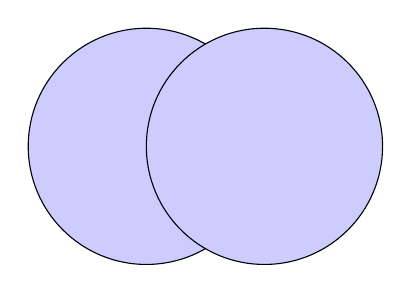
\begin{tikzpicture}
            
            \draw[fill=blue!20] (0,0) circle (1.5);
            \draw[fill=blue!20] (1.5,0) circle (1.5);
            
        \end{tikzpicture}
    \end{center}
    
\end{frame}

\begin{frame}[fragile]{ST\_Union — União}
    
    Combina duas geometrias em uma única.
    
    \begin{minted}{sql}
SELECT ST_Union(geom)
FROM municipios;
    \end{minted}
    
    \begin{center}
        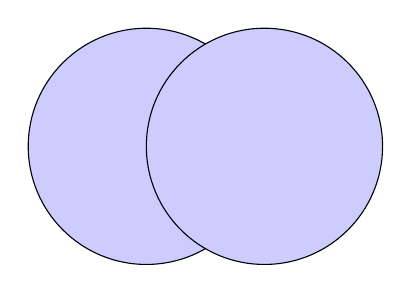
\begin{tikzpicture}
            
            \draw[fill=blue!20] (0,0) circle (1.5);
            \draw[fill=blue!20] (1.5,0) circle (1.5);
            
        \end{tikzpicture}
    \end{center}
    
\end{frame}

\begin{frame}[fragile]{ST\_Difference — Diferença}
    
    Remove de uma geometria a área da outra.
    
    \begin{minted}{sql}
SELECT ST_Difference(a.geom, b.geom)
FROM area_protegida a, rodovia b;
    \end{minted}
    
    \begin{center}
        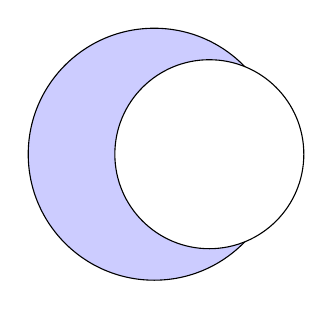
\begin{tikzpicture}
            
            \draw[fill=blue!20] (0,0) circle (1.6);
            \draw[fill=white] (0.7,0) circle (1.2);
            
        \end{tikzpicture}
    \end{center}
    
\end{frame}

\begin{frame}[fragile]{ST\_DWithin — Distância dentro de um limite}
    
    Verifica se duas geometrias estão a uma distância menor ou igual a um valor.
    
    \begin{minted}{sql}
SELECT *
FROM cidades a, hospitais b
WHERE ST_DWithin(a.geom, b.geom, 5000);
    \end{minted}
    
    \vspace{0.3cm}
    
    \textbf{Interpretação:}
    \begin{itemize}
        \item Retorna cidades a até \textbf{5 km} de um hospital
        \item Muito usado em consultas de proximidade
        \item Utiliza \textbf{índices espaciais} quando disponíveis
    \end{itemize}
    
    \begin{center}
        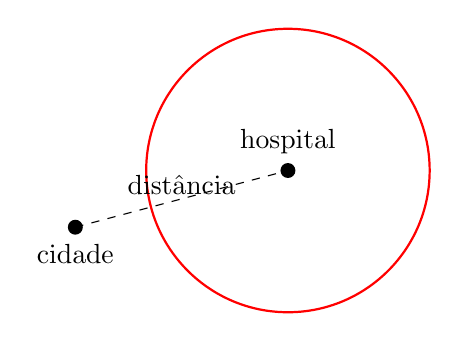
\begin{tikzpicture}[scale=0.9]
            
            % cidade
            \fill (0,0) circle (3pt);
            \node[below] at (0,-0.1) {cidade};
            
            % hospital
            \fill (3,0.8) circle (3pt);
            \node[above] at (3,0.9) {hospital};
            
            % raio de busca
            \draw[red, thick] (3,0.8) circle (2);
            
            % linha distância
            \draw[dashed] (0,0) -- (3,0.8);
            
            \node at (1.5,0.6) {distância};
            
        \end{tikzpicture}
    \end{center}
    
\end{frame}

\end{document}
